\documentclass{article}
\usepackage{tikz}
\usetikzlibrary{patterns}

\begin{document}
  \flushright
  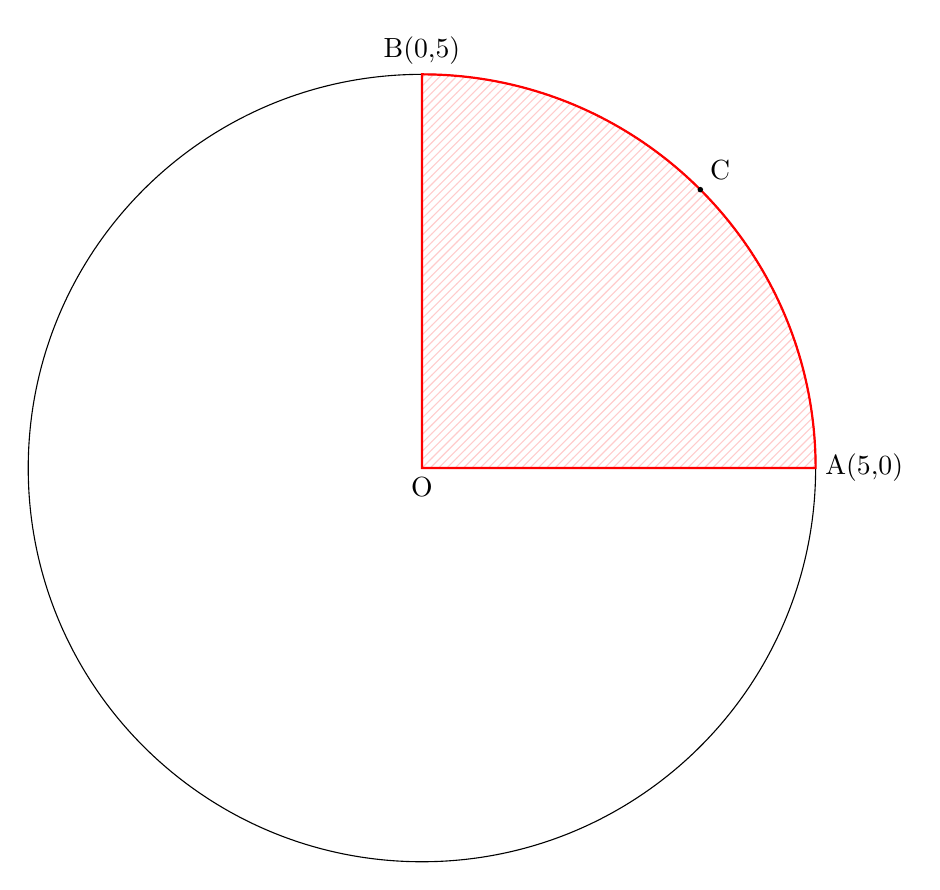
\begin{tikzpicture}
    \def\r{5}
    \draw (0,0) circle (\r); % 绘制一个以(0,0)为圆心,半径为2cm的圆,作为参考
    \node at (0,0)[below] {O};
    \node at (\r,0)[right]{A(\r,0)};
    \node at (0,\r)[above]{B(0,\r)};
    \filldraw[draw=red, pattern=north east lines, pattern color=red!20, thick] (\r,0) arc (0:90:\r cm) -- (0,0) -- cycle; % 绘制圆弧
    \fill (45:\r cm) circle (1pt);
    %\node at (45:5cm) [above right] {C}; 
    \node at (45:\r cm) [anchor = south west] {C}; % anchor = south west
  \end{tikzpicture}
\end{document}
